\documentclass[]{standalone}
\usepackage{tikz}
\begin{document}
  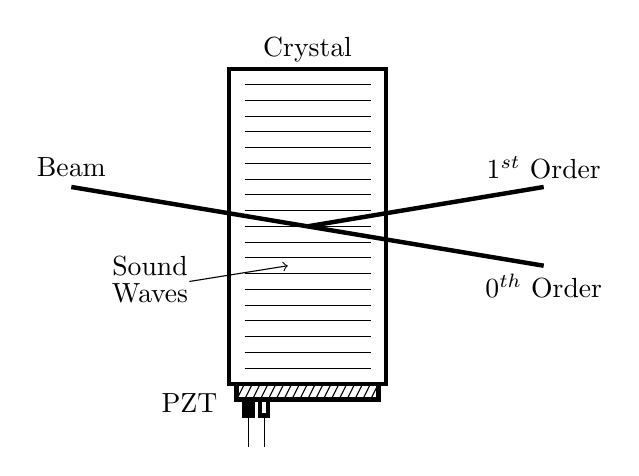
\begin{tikzpicture}
	  \draw[line width = 1.6pt] (-1,-2) rectangle (1,2);
	  \foreach \y in {2,1.8,...,-2}{
		  \draw (-.8,\y) -- (.8,\y);
  }
    \node at (-2,-.5) {Sound};
    \node at (-2,-.85) {Waves};
	\draw[->] (-1.5,-.7) -- (-.25,-.5);
  	\draw[line width = 1.6pt] (-.9,-2) rectangle (.9,-2.2);
  	\draw[line width = 1.6pt,fill = black] (-.8,-2.2) rectangle (-.7,-2.4);
  	\draw[line width = 1.6pt] (-.6,-2.2) rectangle (-.5,-2.4);
	\draw (-.75,-2.4) -- (-.75,-2.8);
	\draw (-.55,-2.4) -- (-.55,-2.8);
	\foreach \d in {0,0.1,...,1.8}
	{
		\draw (-.9 + \d,-2.2) -- (-.9+\d + .1,-2); 
	}

	\node at (0,2.25) {Crystal};
	\node at (-1.5,-2.25) {PZT};

	\draw[line width = 1.6pt] (-3,.5) --(0,0);
	\draw[line width = 1.6pt] (0,0) --(3,.5);
	\draw[line width = 1.6pt] (0,0) --(3,-.5);
	\node at (-3,.75) {Beam};
	\node at (3,.75) {$1^{\text{st}}$ Order};
	\node at (3,-.75) {$0^{\text{th}}$ Order};
  \end{tikzpicture}
\end{document}
